\documentclass[newpage]{homework}
\newcommand{\hwname}{Zooey Nguyen}
\newcommand{\hwemail}{zooeyn@ucla.edu}
\newcommand{\hwclass}{Physics 115A}
\newcommand{\hwtype}{Homework}
\newcommand{\hwnum}{2}
\begin{document}
\maketitle

\question
Normalising with A.
\begin{align*}
    1   &=  \int_{-\infty}^{\infty} Ae^{-\lambda(x-a)^2} \dd{x}
    =	A \sqrt{\frac{\pi}{\lambda}}	\\
    A   &=  \boxed{\sqrt{\frac{\lambda}{\pi}}}
\end{align*}
Finding expectation values.
\begin{align*}
    E(x)	&=	\sqrt{\frac{\lambda}{\pi}}  \int xe^{-\lambda(x-a)^2} \dd{x}
    =  \sqrt{\frac{\lambda}{\pi}}  \left[ \int (x-a)e^{-\lambda(x-a)^2} \dd{x} + \int ae^{-\lambda(x-a)^2} \dd{x} \right]  \\
    &=	\sqrt{\frac{\lambda}{\pi}}  \left[ 0 +  a\sqrt{\frac{\pi}{\lambda}}    \right]
    =	\boxed{a}  \\
    E(x^2)  &=  \sqrt{\frac{\lambda}{\pi}}  \int x^2 e^{-\lambda(x-a)^2} \dd{x}
    =	\sqrt{\frac{\lambda}{\pi}}  \int (u+a)^2 e^{-\lambda u^2} \dd{u}	\\
    &=	\sqrt{\frac{\lambda}{\pi}}  \left[  \int u^2 e^{-\lambda u^2} \dd{u} + 2a \int u e^{-\lambda u^2} \dd{u} + a^2 \int e^{-\lambda u^2} \dd{u} \right] \\
    &=	\sqrt{\frac{\lambda}{\pi}}  \left[  \frac{\sqrt{\pi}}{2\lambda^{3/2}} - 0 + a^2 \sqrt{\frac{\pi}{\lambda}} \right]
    =	\boxed{\frac{1}{2\lambda} - a^2}   \\
    \sigma_x  &=  \sqrt{E(x^2) - E^2(x)}
    =	\sqrt{\frac{1}{2\lambda} - a^2 - (0)^2}
    =	\boxed{\sqrt{\frac{1}{2\lambda} - a^2}}	\\
\end{align*}
Graph of $\rho(x)$.
\begin{figure}[htbp]
    \centering
    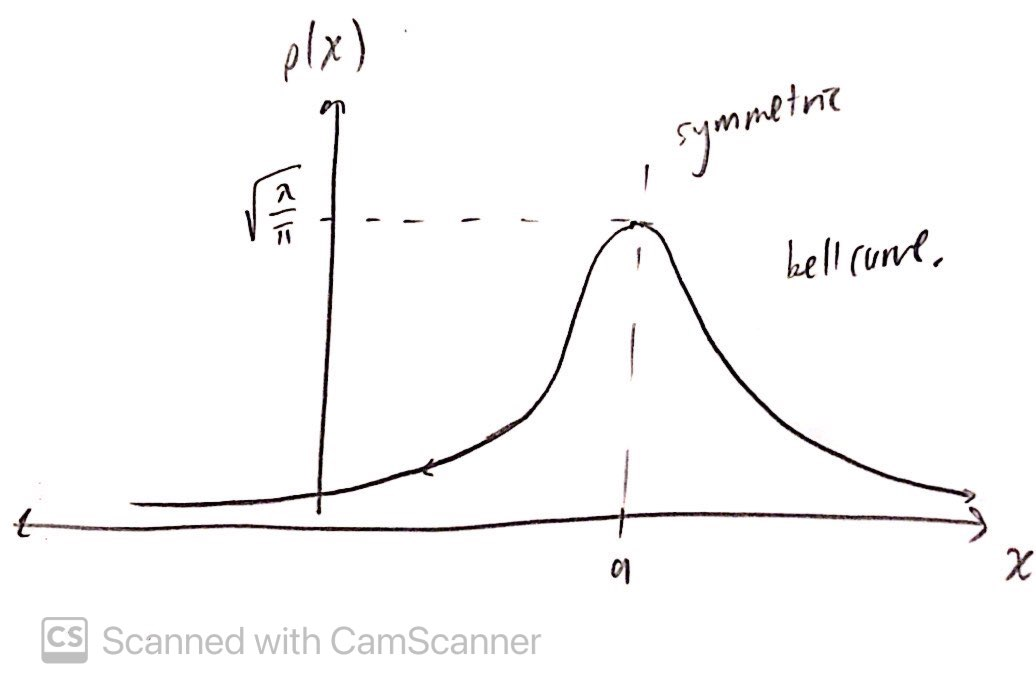
\includegraphics[width=0.6\textwidth]{1c.jpg}
\end{figure}


\question
Normalising with A.
\begin{align*}
    1	&=	\int_0^a (A\frac{x}{a})^2 \dd{x} + \int_a^b (A\frac{b-x}{b-a})^2 \dd{x}	\\
    \frac{1}{A^2}    &=  \int_0^a \frac{x^2}{a^2} \dd{x} + \int_a^b \frac{x^2-2bx+b^2}{(b-a)^2} \dd{x} =	\frac{b}{3}	\\
    A   &=  \boxed{\sqrt{\frac{3}{b}}}
\end{align*}
Graph of $\Psi(x,0)$. The particle is most likely to be found at \fbox{$x=a$} at $t=0$.
\begin{figure}[htbp]
    \centering
    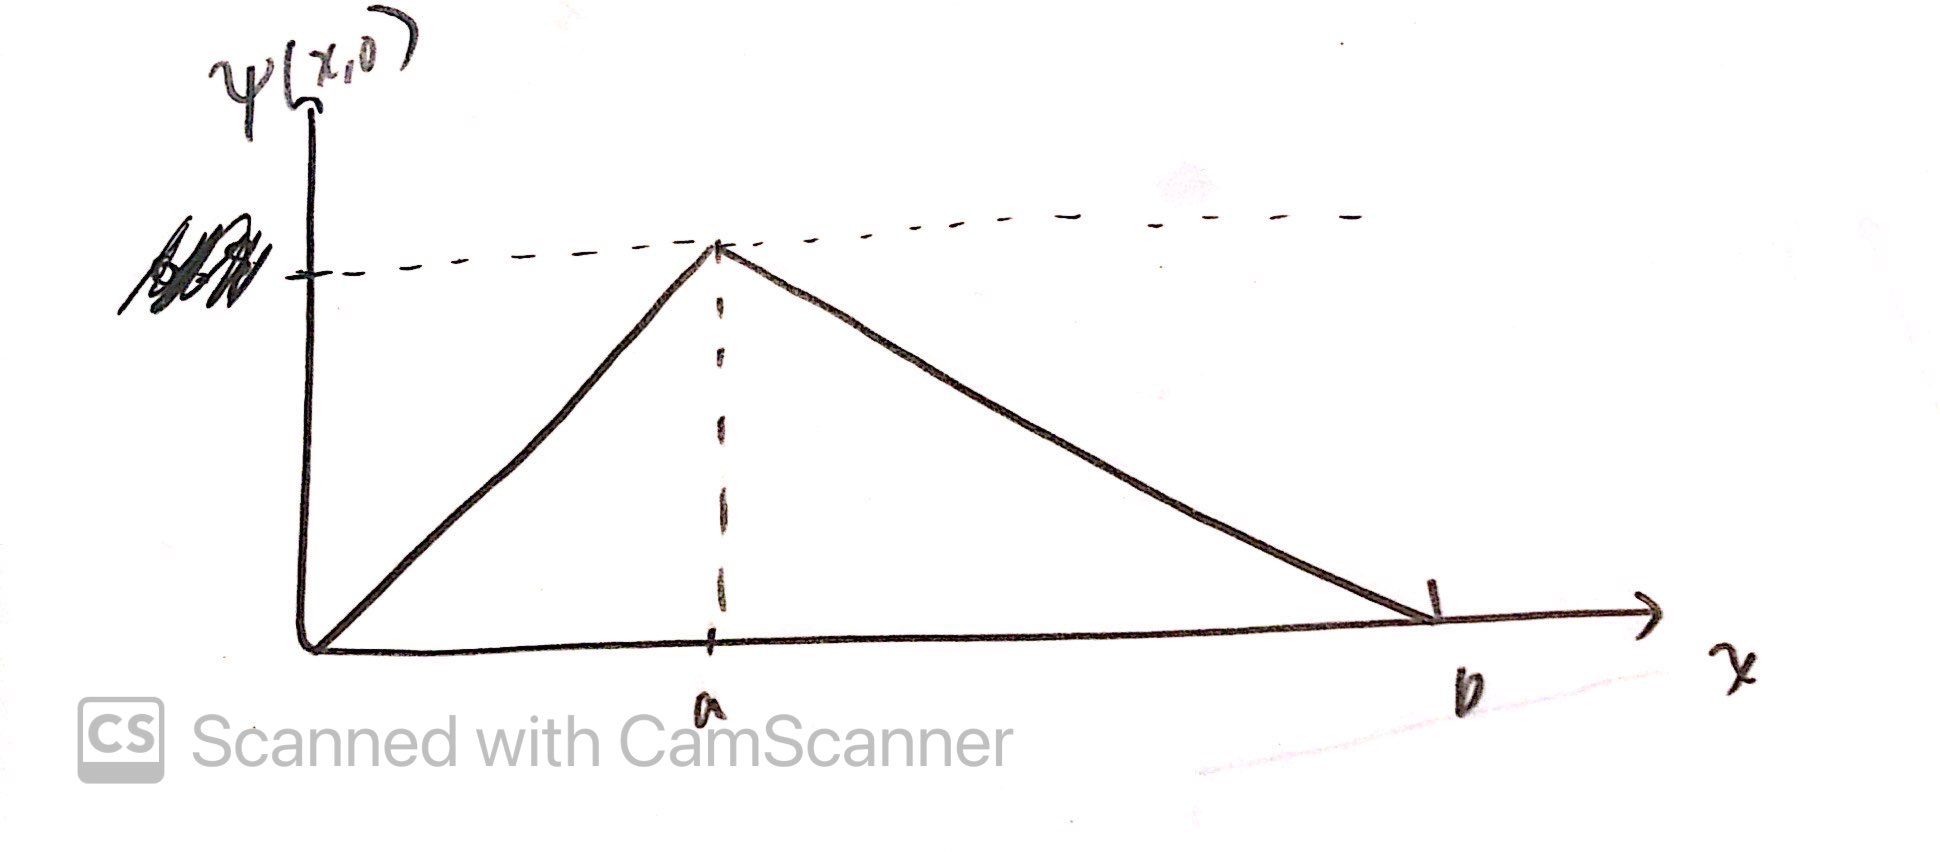
\includegraphics[width=0.6\textwidth]{2b.jpg}
\end{figure}

The probability of finding the particle to the left of a.
\begin{align*}
    P(x < a)	&=	\frac{3}{b} \int_0^a \frac{x^2}{a^2} \dd{x}
    = \boxed{\frac{a}{b}}   \\
    P(x < a)|_{b=a}  &=  1   \\
    P(x < a)|_{b=2a} &=  0.5    \\
\end{align*}
Expectation value of $x$.
\begin{align*}
    E(x)	&=	\frac{3}{b} \left(  \int_0^a \frac{x^3}{a^2} \dd{x} + \int_a^b \frac{x^3-2bx^2+b^2x}{(b-a)^2} \dd{x}  \right)	\\
        &=	\boxed{\frac{2a^3 - 3ba^2 + b^3}{4(b-a)^2}}	\\
\end{align*}

\question
Normalising with A at $t=0$.
\begin{align*}
    1	&=	\int |\Psi(x,0)|^2	\dd{x} = A^2 \int e^{-2\lambda |x|} \dd{x} = \frac{A^2}{\lambda} \\
    A   &=  \boxed{\sqrt{\lambda}}
\end{align*}
Expectation values.
\begin{align*}
    E(x)	&=  \int (\sqrt{\lambda} e^{-\lambda|x|} e^{-i \omega t})[x](\sqrt{\lambda} e^{-\lambda|x|} e^{i \omega t})  \dd{x}
    =  \lambda \int xe^{-2\lambda|x|}  \dd{x}
    = \boxed{0} \\
    E(x^2)  &=  \lambda \int x^2 e^{-2\lambda|x|}  \dd{x}
    = \boxed{\frac{1}{2\lambda^2}}
\end{align*}
Standard deviation.
\begin{align*}
    \sigma	&=	\sqrt{E(x^2) - E^2(x)}	= \boxed{\frac{1}{\lambda\sqrt{2}}}
\end{align*}

\question
Normalising with C.
\begin{align*}
    1	&=	\int_0^\infty [Ce^{-x} (1-e^{-x]})]^2 \dd{x}
    = C^2 \int_0^\infty e^{-2x} (1 - 2e^{-x} + e^{-2x}) \dd{x}  \\
    &=  C^2 [-\frac{e^{-2x}}{2} + \frac{2e^{-3x}}{3} - \frac{e^{-4x}}{4}]_0^\infty
    = \frac{C^2}{12}    \\
    C &= \boxed{2\sqrt{3}}
\end{align*}
Most probable position.
\begin{align*}
    P(x)    &=  12 e^{-2x} (1 - 2e^{-x} + e^{-2x})	\\
    0   &=   \dv{P}{x}   = -24e^{-2x} + 72e^{-3x} - 48e^{-4x}   \\
    0   &=  (e^x)^2 - 3e^x + 2  \\
    e^x &=  (3 \pm \sqrt{9 - 4*2})/2 = 1,2  \\
    P(x=0)  &=  0   \\
    P(x=\ln{2}) &= 0.6931   \\
    x_{max} &=  \boxed{\ln{2}}
\end{align*}
Expectation values. It is higher than the most probable value, which makes sense since the distribution is right-skew, so it is more likely to find it to the right of the mode value than the left of it.
\begin{align*}
    E(x)	&=	\int_0^\infty xP(x) \dd{x}
    = \int_0^\infty 12x e^{-2x} (1 - 2e^{-x} + e^{-2x}) \dd{x} \\
    &= \left[ 12 \left( -\frac{2x+1}{4} e^{-2x}   + \frac{6x+2}{9} e^{-3x} - \frac{4x+1}{16} e^{-4x}   \right)  \right]_0^\infty
    = \boxed{\frac{13}{12}}
\end{align*}

\end{document}
